\chapter{Supplementary Material}
\section{Transforming Raw Data to structured format: Extract, Load, Transform}\label{sec:elt}
Raw data from the experiment is stored in HDF5 files. This includes many \gls{beamline} diagnostic information such as beam arrival monitor (BAM), \gls{GMD}, the delay stage readings, the monochromator energy, sample specific information such as extractor voltage, and the electron counting in the 3 detector dimensions corresponding to the \gls{DLD} spatial $x$ and $y$ axes and the temporal $t_{tof}$. This information is resolved at each bunch of electrons coming from the accelerator called a \gls{train}, which are further microbunched into \glsplural{pulse}.

The Open Community of Multidimensional Photoemission Spectroscopy (OpenCOMPES) was established to develop tools and infrastructure to make analysis easier. To this end, a modular Python library called \texttt{SED} was created that provides the entire pipeline from easy data loading to common calibration and corrections, multidimensional binning to create images, and saving the images to standard formats, with proper care of data provenance.

The data pipeline follows an \gls{ELT} process, wherein raw data is extracted from HDF5 files, transformed into a structured format suitable for analysis, and subsequently stored in intermediate buffer files for further downstream processes such as analysis and visualization.

The following sections provide a detailed exposition of each stage of this \gls{ELT} process, also shown in \cref{fig:elt}. The first stage, extraction, begins with the loading of raw data from the HDF5 files. These files encapsulate experimental results across multiple channels, including electron-resolved and time-resolved data. The hierarchical structure of the HDF5 files allows the organization of data into groups, where each group contains an index and its corresponding dataset, collectively referred to as a “channel” The paths to these HDF5 files, along with relevant configuration parameters, are provided to the pipeline to dictate the steps of the subsequent transformation process.

\subsection*{Pipeline Overview}
To optimize performance and facilitate data management, the pipeline generates buffer files for each type of data (electron and time-resolved). This task is handled by the \texttt{BufferFilePaths} class, which initializes file paths and manages the creation of buffer files in the efficient \texttt{Parquet} format. By checking the presence of pre-existing buffer files, the class determines whether to reuse these files or regenerate them, based on the \texttt{force\_recreate} flag.

Each HDF5 file results in the generation of two primary buffer files: one containing electron-resolved data and another containing pulse/train-resolved data. These files are essential for organizing the data at the pulse level and maintaining resolution at the electron level. The data for each train contains roughly 500 pulses, and although some data is resolved at the pulse level, each index often holds an array, necessitating the use of the \texttt{pandas} MultiIndex functionality to maintain the data’s hierarchical structure. Detector measurements, which are electron-resolved along the X, Y, and temporal axes, are typically represented as three-dimensional arrays and add further complexity to the indexing process.

A critical transformation step involves correcting for offsets in pulse IDs to ensure accurate synchronization of data across different channels. Any data associated with pulse IDs below zero is removed, as it is considered invalid. Similarly, \texttt{NaN} pulses are dropped to avoid introducing inconsistencies in downstream analyses. While it is possible that pulses exceeding 500 may also be invalid, these are not filtered during this stage, as that determination is deferred to the final analysis. Due to machine fluctuations, pulses may become unsorted, and hence the pulses are sorted within each train to maintain temporal order.

Once this cleaning process is completed, electron-resolved channels are combined using an outer join with pulse and train-resolved channels, forming a comprehensive dataframe that contains all relevant information for further analysis. This merged dataset is separated into two primary dataframes: the electron-resolved dataframe and the pulse-resolved dataframe.

The electron dataframe contains only rows where electron events have been detected, with any missing data in non-electron channels forward-filled to ensure completeness. This dataframe serves as the main source of electron-specific data for further analyses. However, given that not all pulses or trains may produce electron events, a separate pulse-resolved dataframe is generated to capture all available train and pulse data, independent of electron detections. This pulse-resolved dataframe is essential for normalization steps involving time-resolved channels, such as those related to the delay axis.

The pipeline also includes validation steps for auxiliary channels, particularly those containing multidimensional data (e.g.\ 4D arrays), ensuring that all required channels exist within the files before proceeding with further transformations.

After this initial transformation and extraction, the buffer files are saved in \texttt{Parquet} format, chosen for its efficiency in storage and speed of access during future computations. The final stage involves the loading of all these buffer files into a unified dataframe using \texttt{Dask}, a distributed computing library that enables scalable processing of large datasets. At this stage, forward-filling is again applied to non-electron channels, ensuring that missing values between files are handled consistently. However, care must be taken when forward-filling across different runs, as this could introduce inter-run inconsistencies.

Finally, the schema of the buffer files is cross-validated against the predefined list of channels to ensure consistency and completeness prior to loading the data into \texttt{Dask}.

\begin{figure}[H]
    \label{fig:elt}
    \centering
    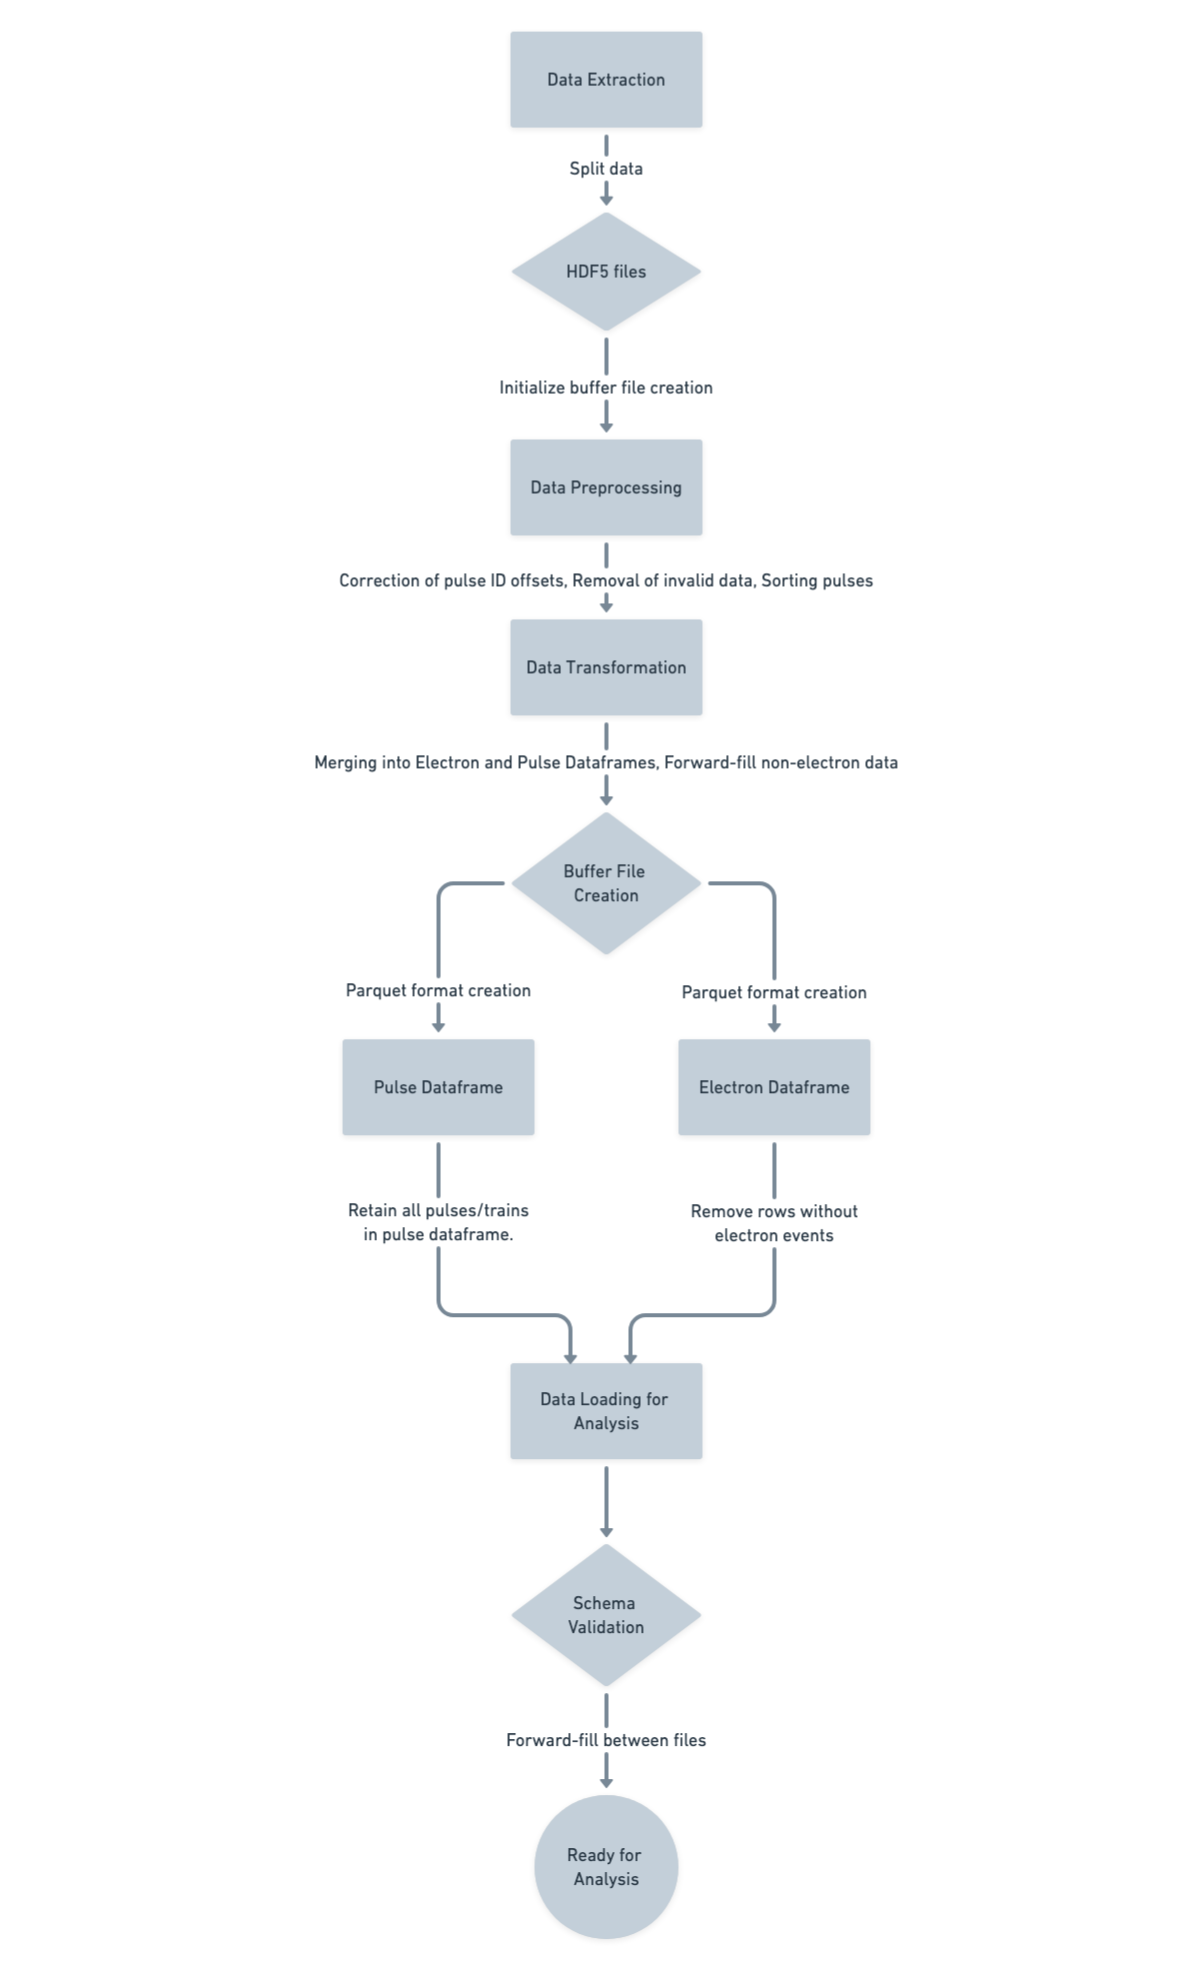
\includegraphics[width=0.7\linewidth]{images/elt_cropped.png}
    \caption{Complete \gls{ELT} pipeline for the data from \gls{HEXTOF} at \gls{FLASH}.}
\end{figure}

\FloatBarrier
\section{Experiment: Metric Comparison}\label{sec:metric_comparison_experiment}

The objective of this experiment is to evaluate the effectiveness of various image quality metrics (\gls{MSE}, \gls{PSNR}, \gls{SSIM}, and \gls{MSSSIM}) when the provided reference is noisy. Specifically, reconstructed images from a trained neural network, that has shown clear improvements in perceptual quality\footnote{This is assessed by an expert and comparing to the high-count target.}, are compared against the high-count but noisy reference. Examples of such images at different counts can be seen in Figure~\ref{fig:images-noisy-denoised-training}, which shows how the noisy images are devoid of any features at low counts, while the denoised images show clear features similar to the target. For this analysis, it is not relevant if the high quality reconstructions are due to overfitting or not, but rather that they produce perceptually better quality images (sometimes even compared to the target). So the hope is that the metrics acknowledge this improvement.

\todo[disable]{As in Chapter 4, I don't see what ``perpetual'' is supposed to mean here.}
\todo[disable]{I don't fully understand what is plotted there. Perhaps you should phrase this as formula so that one can see what exactly is fed into the metrics.}

The \gls{GrIr} dataset is used, with electron counts ranging from \numrange{1e6}{3.2e7}. For each total count, a set of 2D noisy images (referred to as noisy slices) is extracted from the dataset. Corresponding high-count 2D slices (referred to as target slices) are used as reference images for comparison (from the dataset with \num{1.86e8} counts). Likewise, reconstructed images from the neural network are also compared against the target slices.

The metric evaluation procedure involves a data loader, implemented using the \texttt{PyTorch Dataset} class, which iterates through the different datasets and extracts noisy and target 2D image slices (window-averaged or single slice). For each pair of noisy and target slices, the metrics are computed. The comparison results are then grouped by acquisition count and type (noisy vs.\ denoised).

This metric comparison is performed with \num{1638} images sliced along each dimension of the dataset. The results are aggregated and a 95\% confidence interval is calculated for each metric to assess the reliability of the comparison. 
% Table~\ref{tab:comparison_types} summarizes the comparison types and metrics evaluated in this experiment, repeated for both single slice and window-averaged images.
\begin{figure}
    \centering
    \begin{subfigure}[t]{0.48\textwidth}
        \centering
        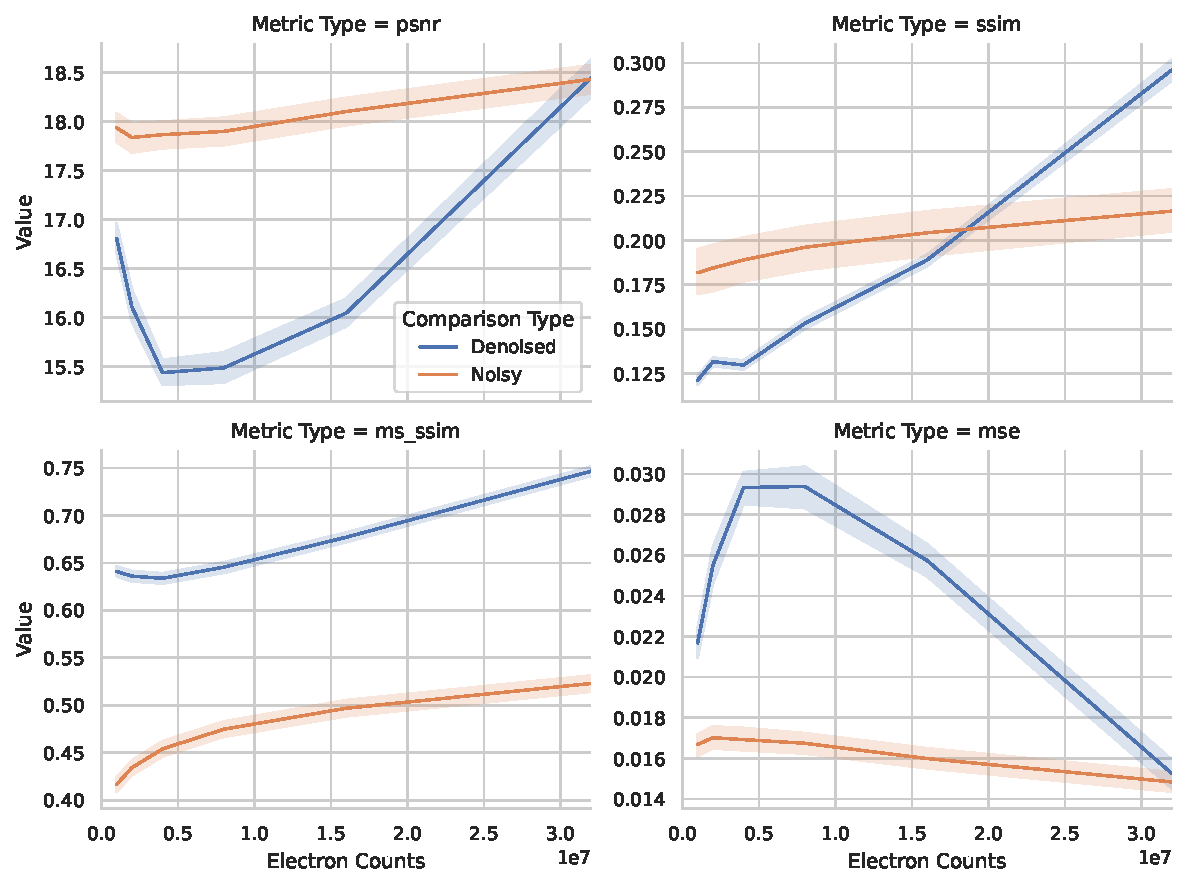
\includegraphics[width=\textwidth]{images/metrics_comparison_denoised_noisy.pdf}
        \caption{Comparison of input and target images window averaged with $w=1$. All metrics improve as counts increase, though \gls{MSE} and \gls{PSNR} show better results for noisy inputs, while \gls{SSIM} and \gls{MSSSIM} favor denoised inputs. \gls{MSSSIM} shows the greatest improvement, indicating it is less sensitive to noise and focused more on perpetual quality.}
        \label{fig:metrics-comparison}
    \end{subfigure}
    \hfill
    \begin{subfigure}[t]{0.48\textwidth}
        \centering
        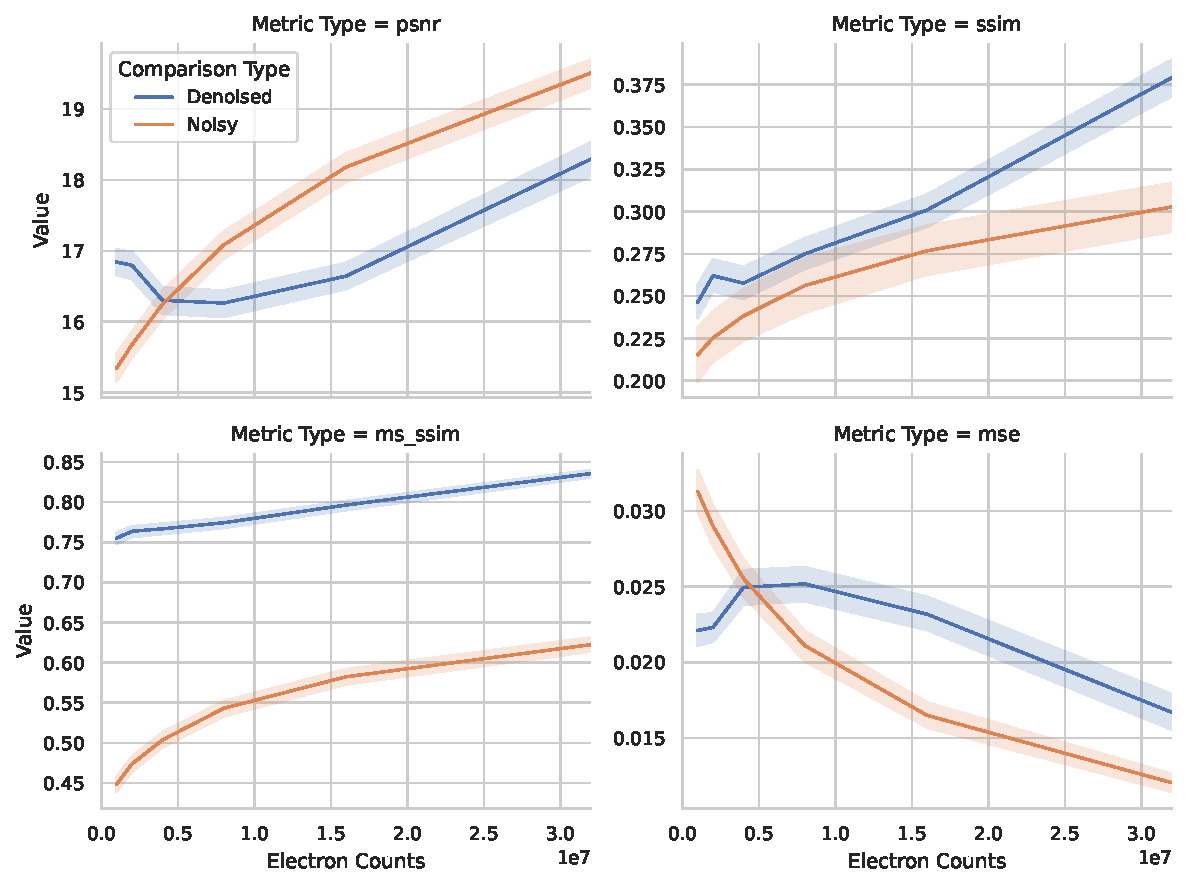
\includegraphics[width=\textwidth]{images/metrics_comparison_denoised_noisy_averaged.pdf}
        \caption{Comparison of input and target images window averaged with $w=1$ and $w=10$, respectively. All metrics improve much faster as counts increase. With a window-averaged target, \gls{MSE} and \gls{PSNR} start to favor the noisy input. \gls{SSIM} shows improvement that the perpetually better images are preferred at all counts. \gls{MSSSIM} exhibits a further separation between noisy and denoised inputs.}
        \label{fig:metrics-comparison-averaged-target}
    \end{subfigure}
    \caption{Evaluation of metrics (\gls{MSE}, \gls{PSNR}, \gls{SSIM}, \gls{MSSSIM}) for noisy and denoised inputs, comparing against noisy input and (less noisy) target slices. The lines show the mean value at each \gls{ncounts}, and the error bands shown in the plots represent a 95\% confidence interval around that mean.}
    \label{fig:combined-metrics-comparison}
\end{figure}

% \begin{figure}[h]
%     \centering
%     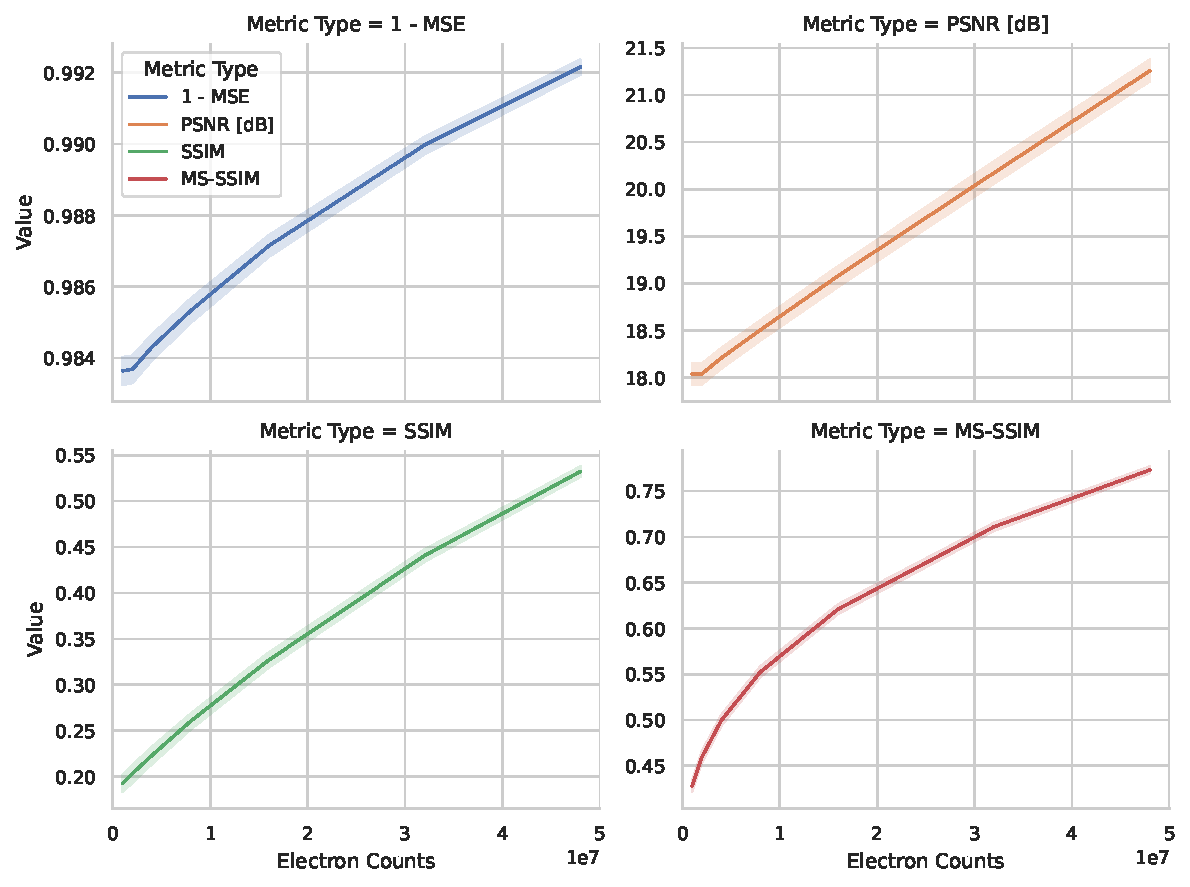
\includegraphics[width=0.7\linewidth]{images/metrics_comparison_same_target.pdf}
%     \caption{Comparison of image quality metrics (\gls{MSE}, \gls{PSNR}, \gls{SSIM}, \gls{MSSSIM}) with noisy realization of a noisy target. The metrics show improved results with increased electron counts, as noise levels decrease. \gls{MSSSIM} shows the best relative improvement in metrics lower counts below \num{e7}.}
%     \label{fig:metrics-comparison-noisy}
% \end{figure}

Comparing the noisy images with target, all metrics trivially show an improvement with increased counts (less noise) (see \cref{fig:metrics-comparison}). However, \gls{MSE}, \gls{PSNR} and \gls{SSIM} show deteriorated metrics when comparing against perpetually high quality images. This can be attributed to the presence of noise in the reference image. For higher counts, \gls{SSIM} manages to show improved results, whereas \gls{MSE} and \gls{PSNR} report consistently worse results compared to the noisy images. \gls{MSSSIM} consistently reports better results with the higher quality images, making it the most reliable metric for evaluation.

% \begin{figure}
%     \centering
%     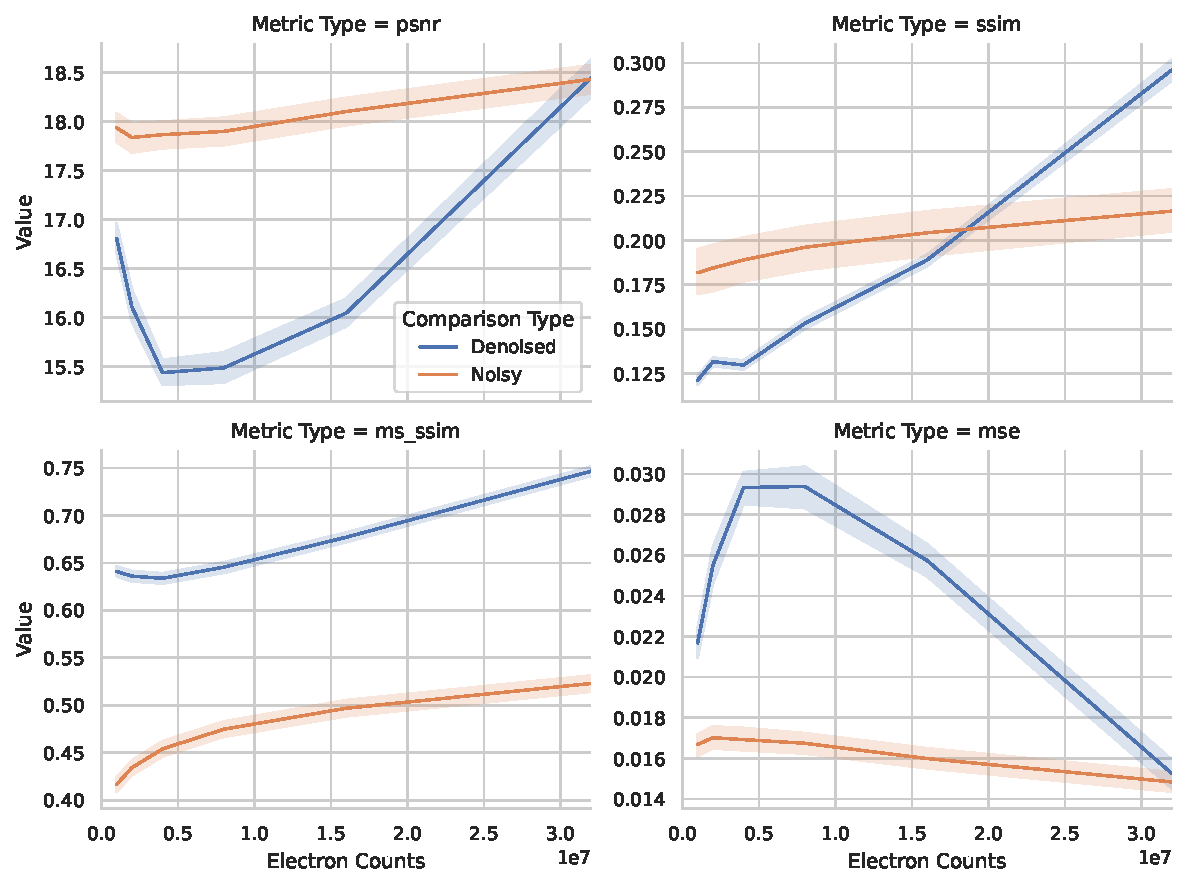
\includegraphics[width=0.7\linewidth]{images/metrics_comparison_denoised_noisy.pdf}
%     \caption{Shows comparison of evaluating metrics (\gls{MSE}, \gls{PSNR}, \gls{SSIM}, \gls{MSSSIM}) with the input being a noisy realization of target or denoised version of that realization. Both are compared to a high-count target that is also noisy. Trivially, all metrics show an improvement when the counts increase. However, \gls{MSE} and \gls{PSNR} evaluate better when the input is noisy, while \gls{SSIM} and \gls{MSSSIM} show better results when the input is denoised. The gap between noisy and denoised is more pronounced for \gls{MSSSIM} than \gls{SSIM}, hence the better metric. }
%    \label{fig:metrics-comparison}
% \end{figure}

% \begin{figure}
%     \centering
%     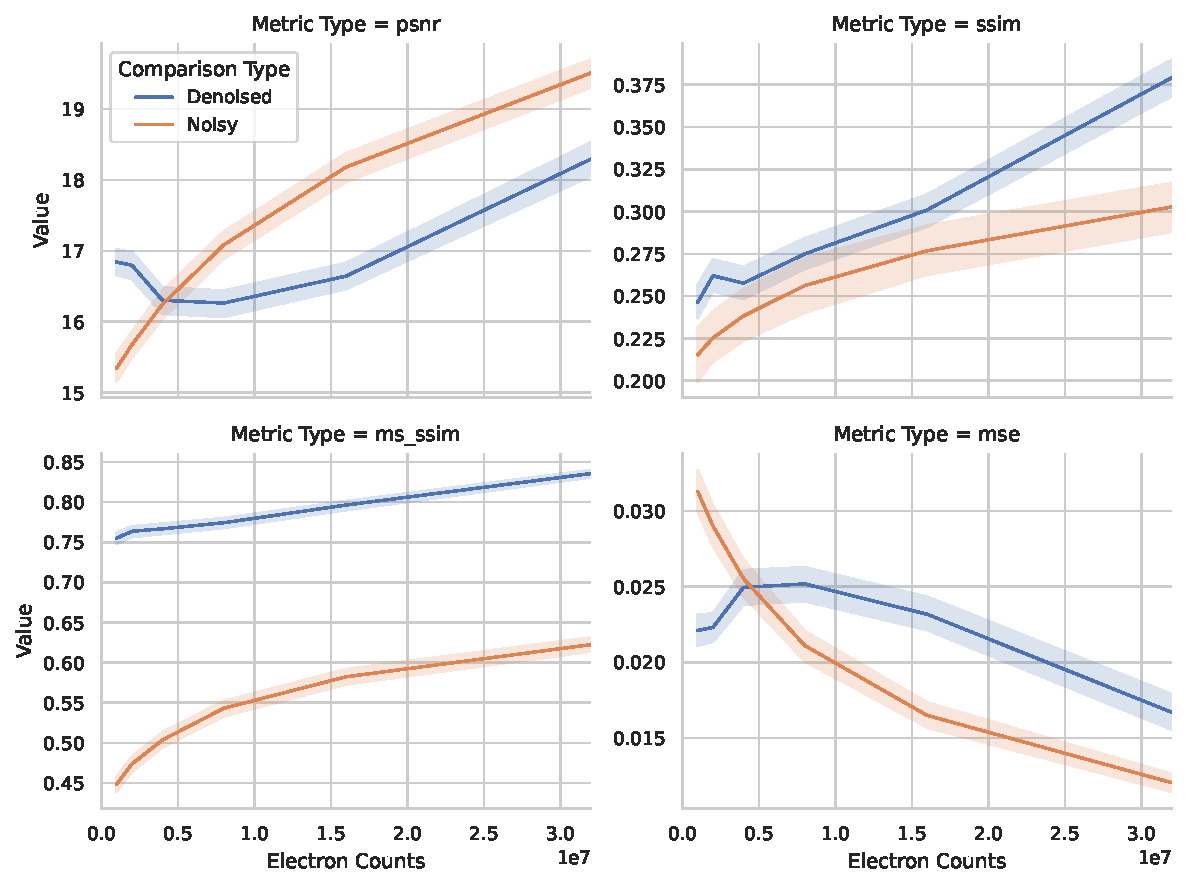
\includegraphics[width=0.7\linewidth]{images/metrics_comparison_denoised_noisy_averaged.pdf}
%     \caption{Metrics comparison for noisy 2D slices against a window-averaged target slice. For \gls{MSE} and \gls{PSNR}, the window-averaged target lowers the reported metrics. \Gls{SSIM} shows a small improvement over the noisy target, while \gls{MSSSIM} shows a large improvement.}
%     \label{fig:metrics-comparison-averaged-target}
% \end{figure}

Additionally, we investigate the effect of window-averaged reference images on the metrics. Results in \cref{fig:metrics-comparison-averaged-target} indicate that window-averaged image as reference generally makes the metric prefer the noisy realization, except in the case of \gls{SSIM} and \gls{MSSSIM}, in the latter of which the gap between the metrics calculated with noisy and high quality images split up further. Consequently, we adopt the window-averaged images as reference for the denoising evaluation.

\FloatBarrier
\section{Deep Learning Infrastructure}
Model Architecture: UNET 2D and 3D

Trained on A100 GPU 80 GB using Maxwell Cluster at DESY. 

\FloatBarrier
\section{Supplementary Figures for Deep Learning based Denoising}
\begin{figure}[h]
    \centering
    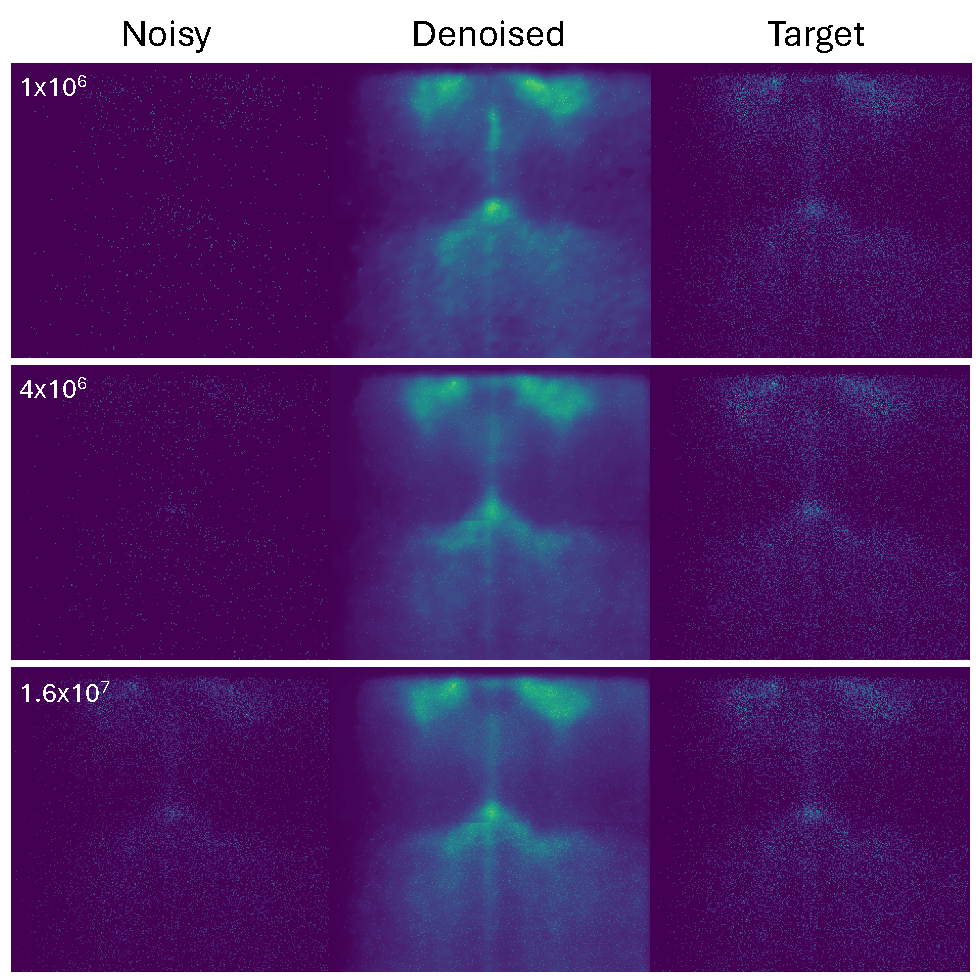
\includegraphics[width=1\linewidth]{images/nn_denoised_ex_single_slice.pdf}
    \caption{Noisy, denoised, and target \gls{E}-\gls{kx} cuts with window size $w=1$ shown for \gls{GdW} dataset. Each row corresponds \numlist{1e6;4e6;1.6e7} counts, respectively.}
    \label{fig:nn-denoised-ex-single-slice}
\end{figure}

\begin{figure}[h]
    \centering
    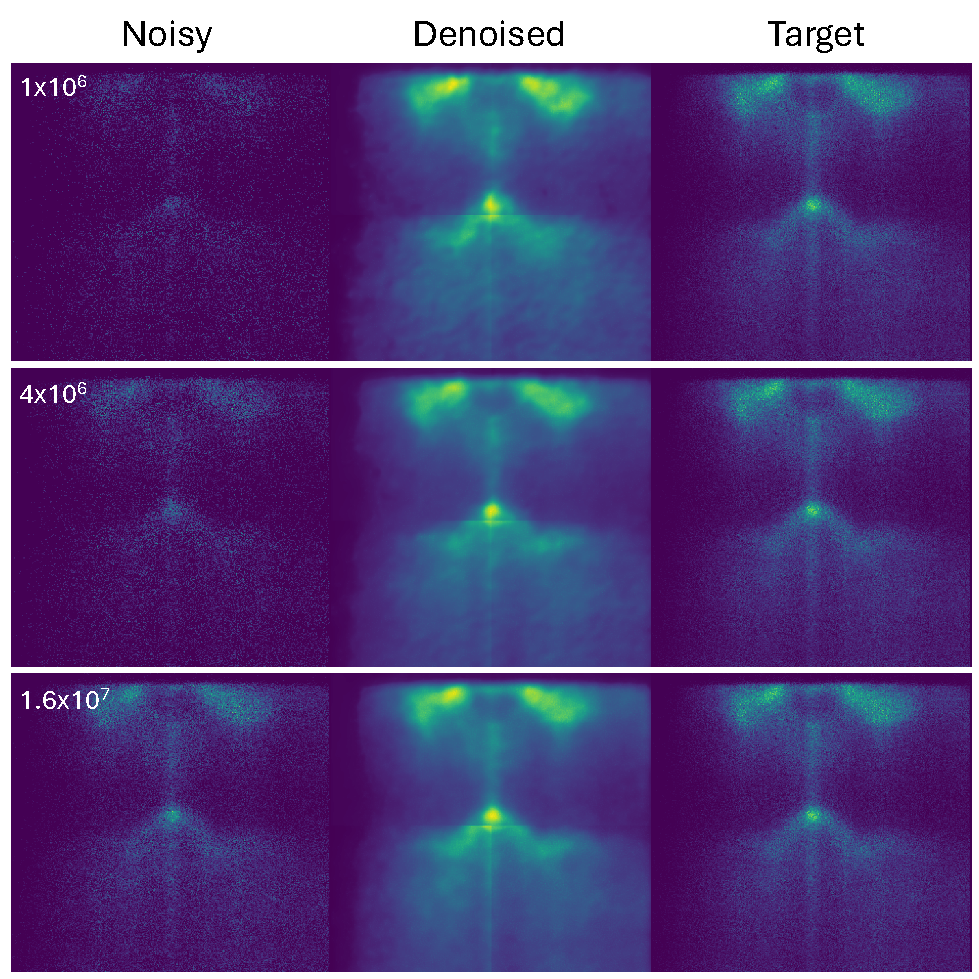
\includegraphics[width=1\linewidth]{images/nn_denoised_ex_20_slice.pdf}
    \caption{Noisy, denoised, and target \gls{E}-\gls{kx} cuts with window size $w=20$ shown for \gls{GdW} dataset. Each row corresponds \numlist{1e6;4e6;1.6e7} counts, respectively.}
    \label{fig:nn-denoised-ex-20-slice}
\end{figure}

\begin{figure}[h]
    \centering
    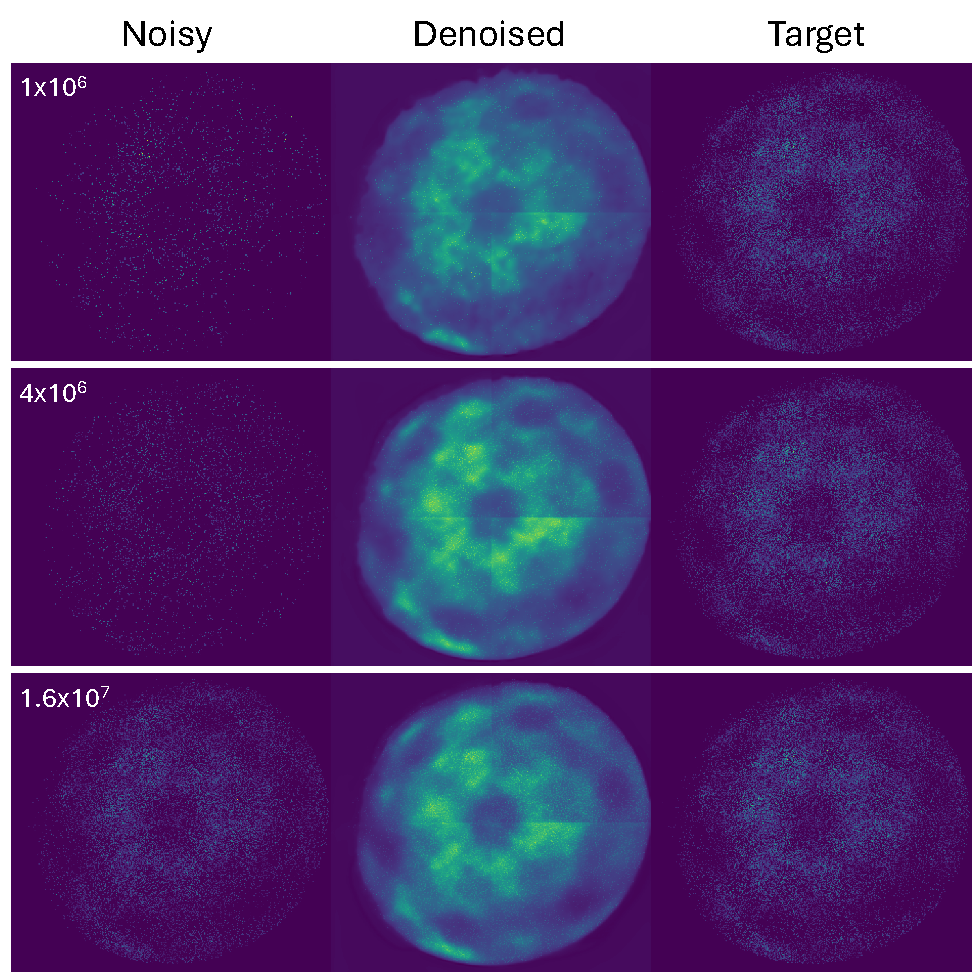
\includegraphics[width=1\linewidth]{images/nn_denoised_xy_single_slice.pdf}
    \caption{Noisy, denoised, and target \gls{ky}-\gls{kx} cuts with window size $w=1$ shown for \gls{GdW} dataset. Each row corresponds \numlist{1e6;4e6;1.6e7} counts, respectively.}
    \label{fig:nn-denoised-xy-single-slice}
\end{figure}

\begin{figure}[h]
    \centering
    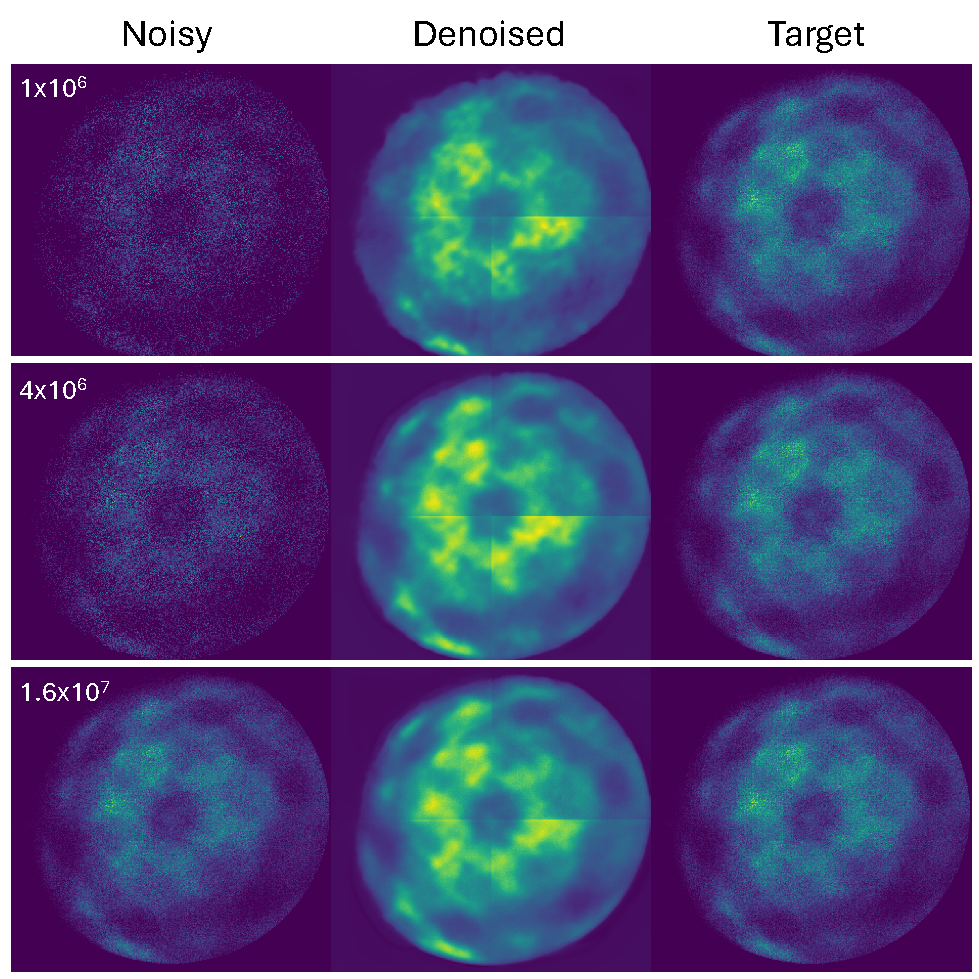
\includegraphics[width=1\linewidth]{images/nn_denoised_xy_20_slice.pdf}
    \caption{Noisy, denoised, and target \gls{ky}-\gls{kx} cuts with window size $w=20$ shown for \gls{GdW} dataset. Each row corresponds \numlist{1e6;4e6;1.6e7} counts, respectively.}
    \label{fig:nn-denoised-xy-20-slice}
\end{figure}

\FloatBarrier
\section{Supplementary Figures for Photoelectron Counting Statistics}
The following section outlines the counting statistics observed for \gls{PES} at two different light sources: a pulsed laser (\gls{WSe2} dataset), and a \gls{SASE} \gls{FEL} light source (\gls{GrIr} dataset). 

\cref{fig:wse2-stats-2} shows the distribution of photoelectron counts for different time intervals ($\Delta t$) within a volumetric subset of the full \gls{WSe2} dataset. The count distributions for smaller time intervals ($\Delta t = \qtylist{2;10;20}{ms}$) follow Poisson statistics, as expected from an uncorrelated photoemission process where spatial and temporal fluctuations are minimal. However, for longer time intervals ($\Delta t = \qty{50}{ms}$), the distribution starts to deviate from the Poisson distribution. This deviation suggests that spatial correlations, due to the material properties of the sample, become significant enough to impact the distribution. While the impact of pulse light source should be minimal since the time intervals we look at are much longer than the pulse durations, the spatial correlations could be due to the material properties of the sample.


The \gls{GrIr} dataset reveals more complex photoelectron count statistics over a broader range of time intervals. Figures \ref{fig:grir-stats-1}, \ref{fig:grir-stats-2}, and \ref{fig:grir-stats-3} show photoelectron count distributions for varying time windows ($\Delta t = \qtylist{10;50;100;500;1000;5000}{ms}$) in the acquisition time $T\approx\qty{30}{hour}$


\begin{figure}
    \centering
    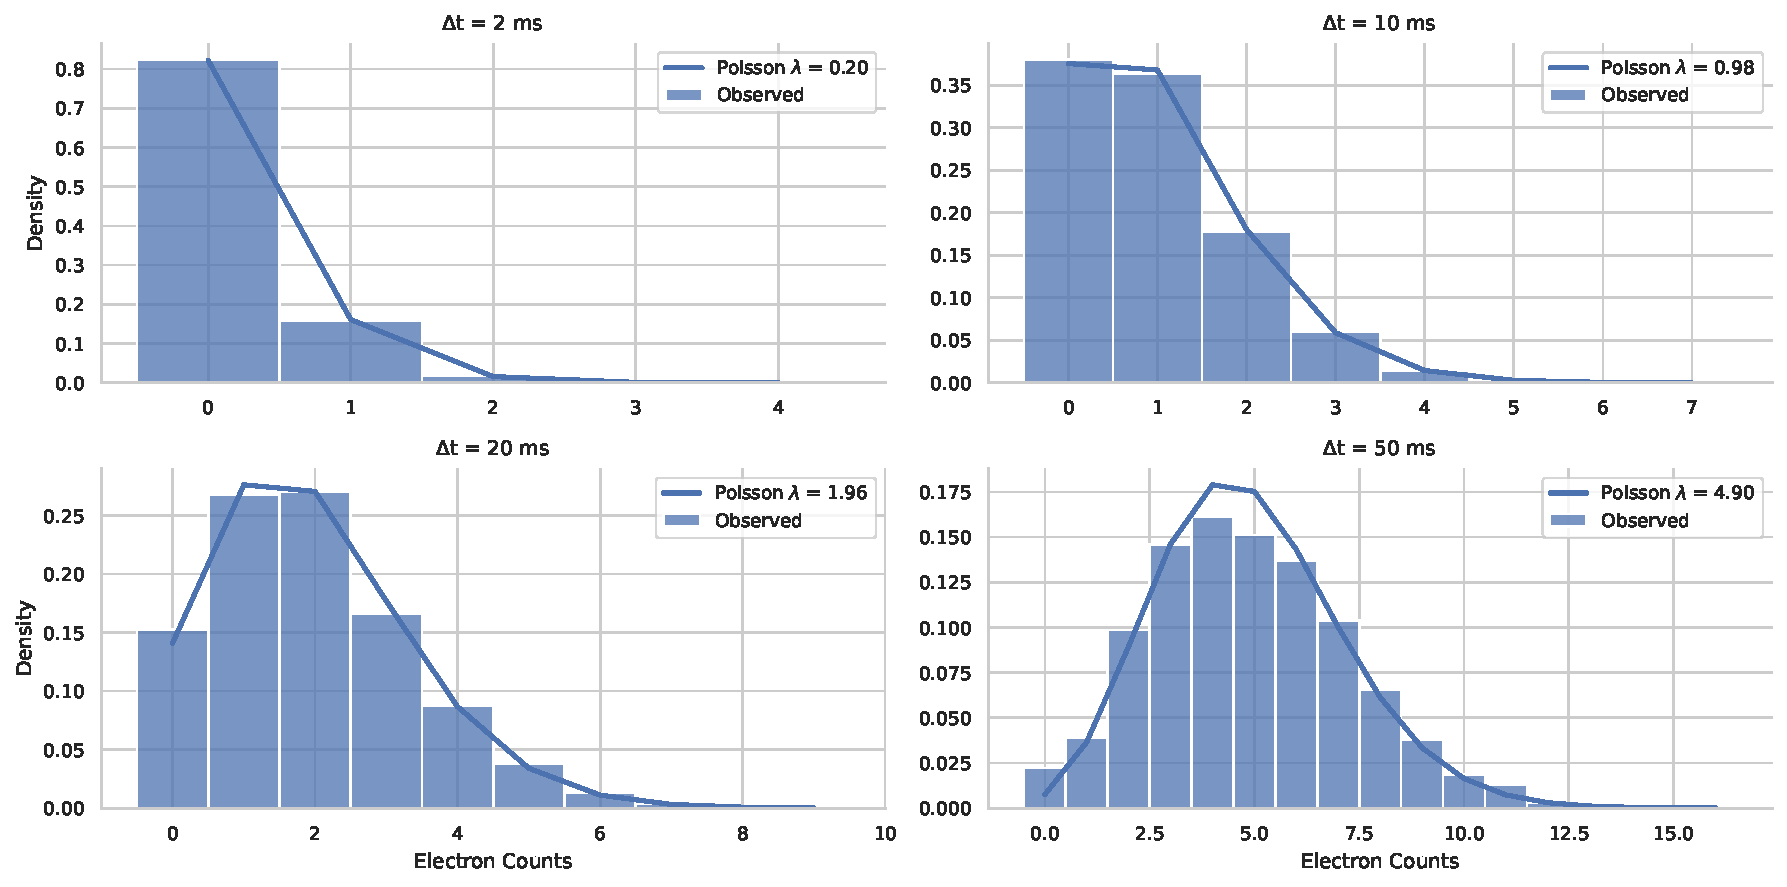
\includegraphics[width=1\linewidth]{images/hist_counts_facetgrid_2_wse2.pdf}
    \caption{Distribution of photoelectron counts at time intervals $\Delta t =$ \qtylist{2;10;20;50}{ms} for a different volumetric subset of the full \gls{WSe2} dataset. Poisson statistics are observed at smaller time intervals, but as the time window increases ($\Delta t =$ \qty{50}{ms}), the data starts to deviate from the Poisson distribution, as spatial correlations become apparent.}
    \label{fig:wse2-stats-2}
\end{figure}

\begin{figure}
    \centering
    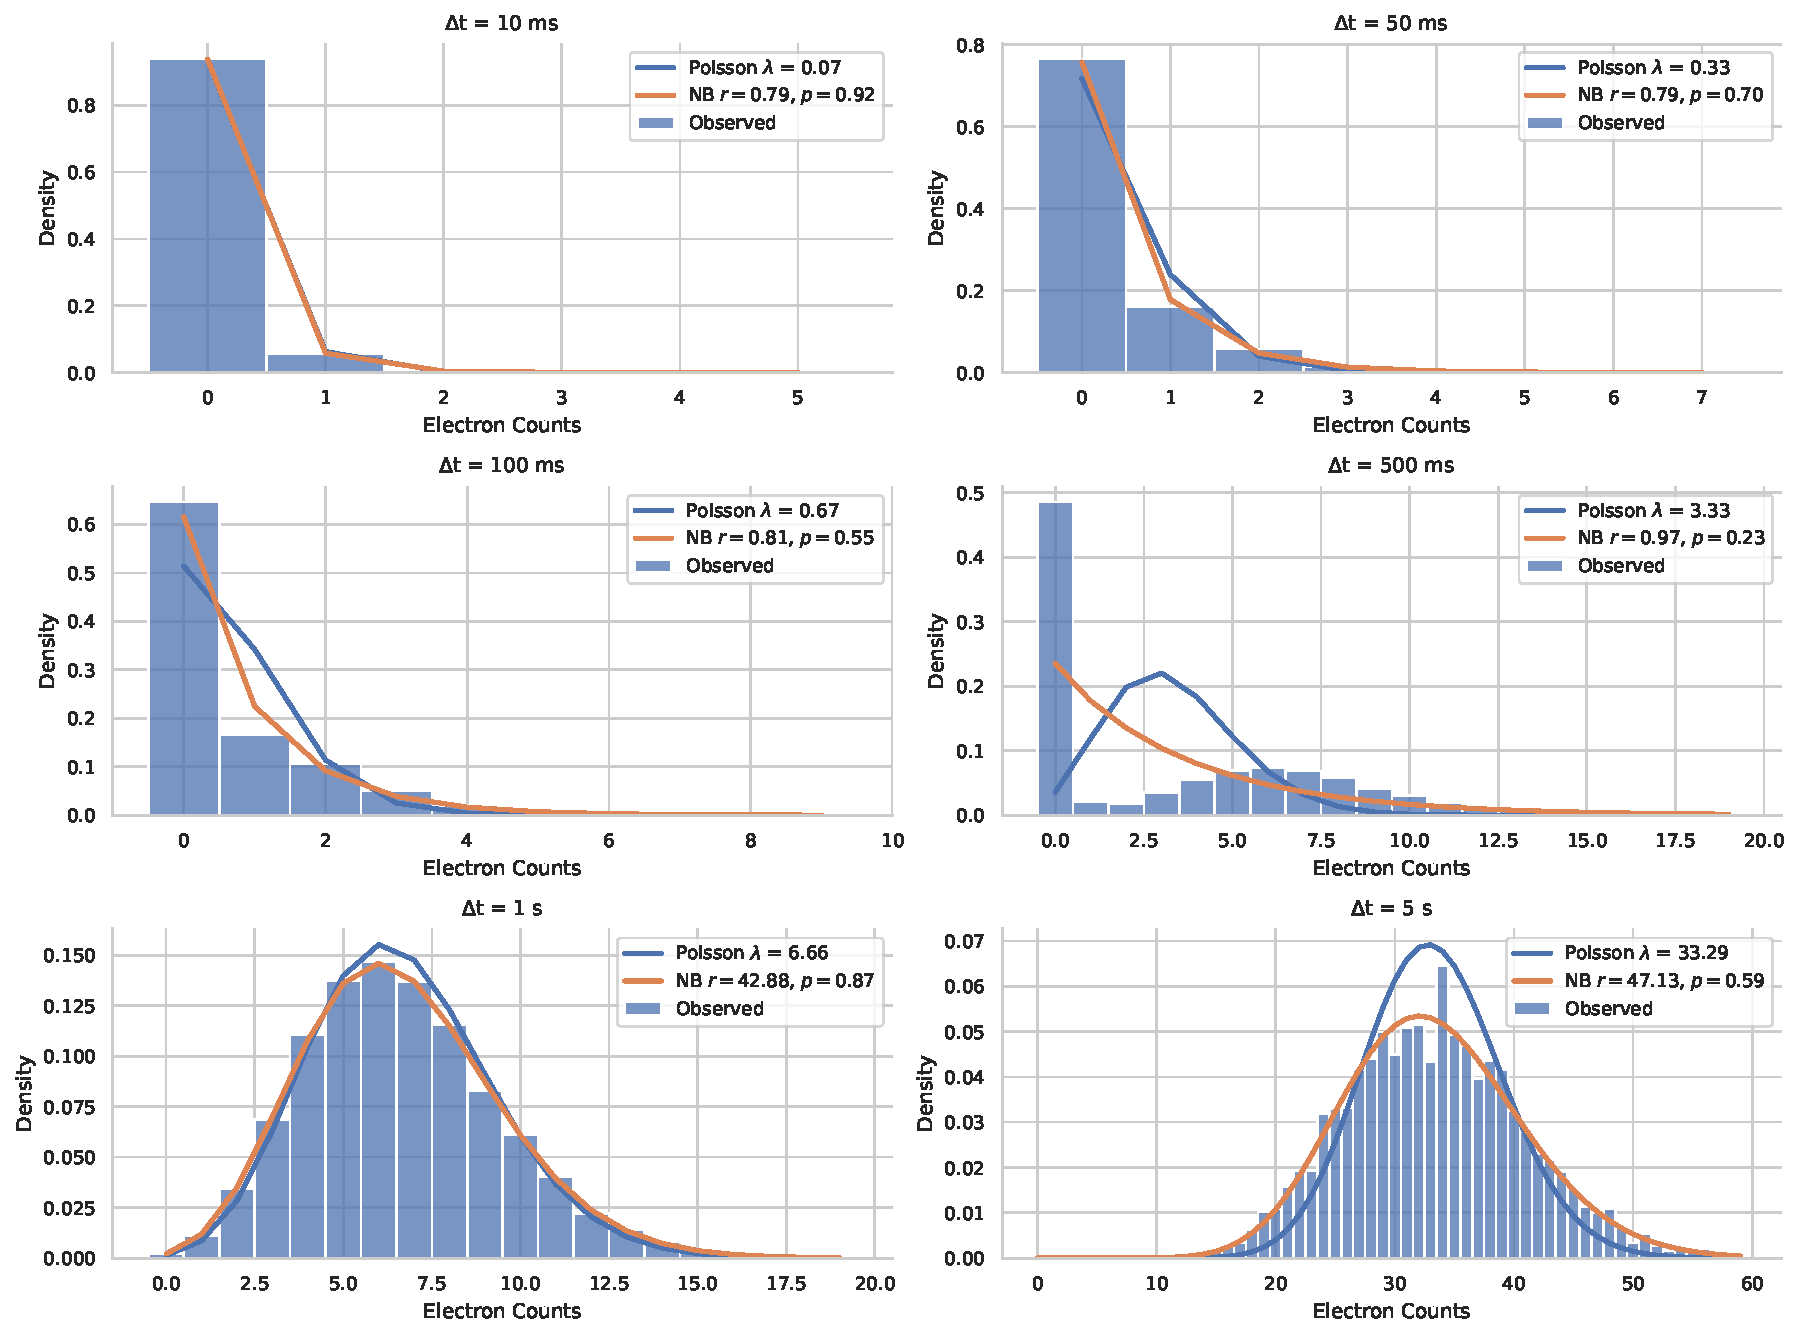
\includegraphics[width=1\linewidth]{images/hist_counts_facetgrid_3_grir.pdf}
    \caption{Distribution of photoelectron counts at time intervals $\Delta t =$ \qtylist{10;50;100;500;1000;5000}{ms} for a selected volumetric subset of the full \gls{GrIr} dataset. Poisson statistics provide a good fit at $\Delta t \leq \qty{100}{ms}$. However, for intervals $\Delta t =$ \qtylist{0.5;1;5}{s} the distribution exhibits over dispersion with a right-skewed tail, characteristic of the \gls{NB} distribution. The total counts in this selected region are $\gls{ncounts}=\num{1e6}$ with total observation time $T\approx\qty{4}{h}$  (See red region in \cref{fig:gmd-intensity}). The smaller $\Delta t$ values may represent the limiting case of the \gls{NB} distribution approaching Poisson statistics.}
    \label{fig:grir-stats-3}
\end{figure}
% \subsection{Mathematical Formulation}
% As shown in \cref{alg:bm3d} and \cref{fig:bm3d-schematic}, the \gls{BM3D} scheme is a two-stage image denoising algorithm that exploits non-local image similarities. The algorithm processes a noisy image $X$ to produce a denoised estimate $\hat{Y}$ through collaborative filtering of similar patches.

% Stage 1: Basic Estimate

% The first stage produces a basic estimate through the following steps:

% 1. **Block Matching**: For each reference block $B_r$ of size $N_1 \times N_1$ in the noisy image, similar blocks are found using the normalized $l^2$-distance:
   
%    $$d(B_r, B_k) = \frac{\|B_r - B_k\|_2^2}{N_1^2}$$

%    Blocks with distance below a threshold $\tau_{\text{match}}$ are grouped:
   
%    $$\mathcal{S}(B_r) = \{B_k : d(B_r, B_k) \leq \tau_{\text{match}}\}$$

% 2. **3D Block Formation**: Similar blocks are stacked into a 3D array $\mathcal{Z}$ of size $N_1 \times N_1 \times |\mathcal{S}(B_r)|$:
   
%    $$\mathcal{Z} = [B_r | B_{k_1} | B_{k_2} | ... | B_{k_n}]$$

% 3. **3D Transform**: A separable 3D transform $\mathcal{T}_{3D}$ is applied:
   
%    $$\mathcal{T}_{3D} = \mathcal{T}_{2D} \otimes \mathcal{T}_{1D}$$
   
%    where $\mathcal{T}_{2D}$ is typically a 2D DCT applied to each block, and $\mathcal{T}_{1D}$ is a 1D Haar transform along the similarity dimension.

% 4. **Hard Thresholding**: The transform coefficients are hard-thresholded:
   
%    $$\Gamma_{\lambda_{\text{3D}}}(\mathcal{T}_{3D}\mathcal{Z}) = 
%    \begin{cases} 
%    (\mathcal{T}_{3D}\mathcal{Z})_{i,j,k} & \text{if } |(\mathcal{T}_{3D}\mathcal{Z})_{i,j,k}| > \lambda_{\text{3D}} \\
%    0 & \text{otherwise}
%    \end{cases}$$

% 5. **Inverse Transform and Aggregation**: The filtered blocks are transformed back and aggregated with weights $w_{B_r}$ based on the number of non-zero coefficients after thresholding:
   
%    $$\hat{Y}_{\text{basic}} = \frac{\sum_{B_r} w_{B_r} \cdot \mathcal{T}_{3D}^{-1}(\Gamma_{\lambda_{\text{3D}}}(\mathcal{T}_{3D}\mathcal{Z}))}{\sum_{B_r} w_{B_r}}$$

% Stage 2: Final Estimate

% The second stage uses the basic estimate to perform Wiener filtering:

% 1. **Block Matching**: In the second stage, the block matching uses both the noisy image $X$ and the basic estimate $\hat{Y}_{\text{basic}}$. The distance between blocks is computed as:
% $$d_2(B_r, B_k) = |B_r^{\text{basic}} - B_k^{\text{basic}}|2^2 = \sum{i,j} (B_r^{\text{basic}}[i,j] - B_k^{\text{basic}}[i,j])^2$$
% where $B_r^{\text{basic}}$ and $B_k^{\text{basic}}$ are blocks from the basic estimate $\hat{Y}_{\text{basic}}$. The grouping in the second stage creates a set:
% $$B = {B_k : d_2(B_r, B_k) \leq \tau_2}$$
% where $\tau_2$ is the threshold for the second stage. The corresponding blocks from the noisy image $X$ are then used for the actual Wiener filtering, but their grouping is determined by the similarity of blocks in the basic estimate.
% This approach is more reliable than using the noisy image alone because the basic estimate has reduced noise, leading to more accurate block matching.

% 2. **Wiener Filtering**: For each 3D group $\mathcal{Z}$, the Wiener shrinkage coefficients are:

%    $$W_{i,j,k} = \frac{|(\mathcal{T}_{3D}\mathcal{Z}_{\text{basic}})_{i,j,k}|^2}{|(\mathcal{T}_{3D}\mathcal{Z}_{\text{basic}})_{i,j,k}|^2 + \sigma^2}$$

%    where $\mathcal{Z}_{\text{basic}}$ is the corresponding group from $\hat{Y}_{\text{basic}}$ and $\sigma^2$ is the noise variance.

% 3. **Final Estimate**: The final estimate is obtained by:

%    $$\hat{Y} = \frac{\sum_{B_r} w_{B_r} \cdot \mathcal{T}_{3D}^{-1}(W \cdot \mathcal{T}_{3D}\mathcal{Z})}{\sum_{B_r} w_{B_r}}$$

% This two-stage approach is particularly effective because the Wiener filter coefficients are computed using the basic estimate, which provides a more reliable power spectrum estimate than the noisy image alone.
% \begin{algorithm}
%     \caption{BM3D Denoising Algorithm}\label{alg:bm3d}
%     \begin{algorithmic}[1]
%     \Require Noisy image $X$, noise variance $\sigma^2$
%     \Ensure Denoised image $\hat{Y}$
%     \Statex
%     \State // Stage 1: Basic Estimate
%     \State $\hat{Y}_{\text{basic}} \gets \textsc{BasicEstimate}(X, \sigma^2)$
%     \State // Stage 2: Final Estimate
%     \State $\hat{Y} \gets \textsc{WienerFiltering}(X, \hat{Y}_{\text{basic}}, \sigma^2)$
%     \State \textbf{return} $\hat{Y}$
%     \end{algorithmic}
% \end{algorithm}

% \begin{algorithm}
%     \caption{Basic Estimate}\label{alg:basicestimate}
%     \begin{algorithmic}[1]
%     \Require Noisy image $X$, noise variance $\sigma^2$
%     \Ensure Basic estimate $\hat{Y}_{\text{basic}}$
%     \For{each reference block $B_r$ in $X$}
%         \State $\mathcal{S}(B_r) \gets \{B_k : d(B_r, B_k) \leq \tau_{\text{match}}\}$ \Comment{Block matching}
%         \State $\mathcal{Z} \gets \text{Stack}(B_r, \mathcal{S}(B_r))$ \Comment{3D array formation}
%         \State $\mathcal{T}_{3D}\mathcal{Z} \gets \textsc{3DTransform}(\mathcal{Z})$
%         \State $\mathcal{Z}_{\text{filtered}} \gets \Gamma_{\lambda_{\text{3D}}}(\mathcal{T}_{3D}\mathcal{Z})$ \Comment{Hard thresholding}
%         \State $\mathcal{Z}_{\text{spatial}} \gets \textsc{3DInverseTransform}(\mathcal{Z}_{\text{filtered}})$
%         \State Update $\hat{Y}_{\text{basic}}$ with weighted $\mathcal{Z}_{\text{spatial}}$
%     \EndFor
%     \State \textbf{return} $\hat{Y}_{\text{basic}}$
%     \end{algorithmic}
% \end{algorithm}